\chapter{GEOMETRIC COMPUTATION NATURE}
\label{chap:chap-three}

\section{To Cover Users}
{\bfseries Definition 3.} The $k_{th}$ score $S_{ik}$ represents the scores 
to ranks top-k corresponding to user $w_i$. 

For simplicity, we mark 
\begin{enumerate}
    \item $w_i\cdot p=S_{ik}$ as $h_i$
    \item $w_i\cdot p>S_{ik}$ as $h_i^+$
    \item $w_i\cdot p<S_{ik}$ as $h_i^-$
\end{enumerate}

\begin{figure}[hbt!]
  \centering
  \begin{subfigure}[b]{0.45\linewidth}
    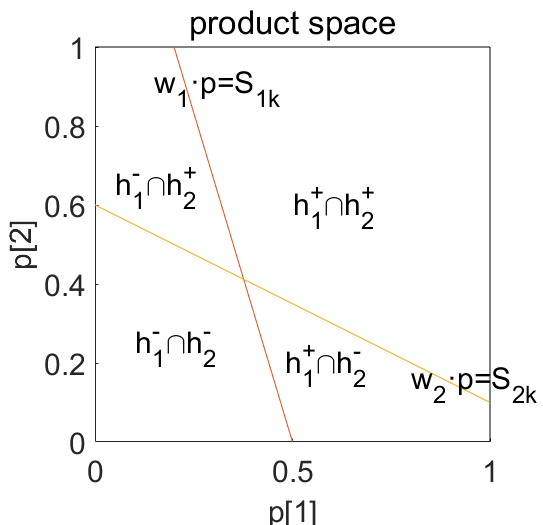
\includegraphics[width=\linewidth]{the_hp_insertion.png}
    \caption{Hyper-plane insertion}
    \label{the_hp_insertion}
  \end{subfigure}
  %
  \begin{subfigure}[b]{0.45\linewidth}
    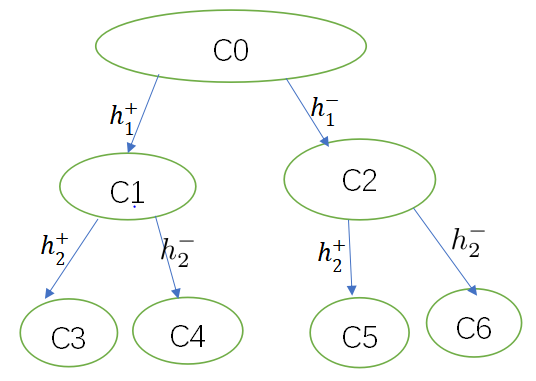
\includegraphics[width=\linewidth]{f2.png}
    \caption{$CellTree$ insertion}
    \label{cell_tree_nodes}
  \end{subfigure}
  \caption{hyper-plane insertion and $CellTree$ insertion}
\end{figure}

As shown in Figure \ref{the_hp_insertion}, when it comes to multiple users, 
such as 2 users
 $\{w_1, w_2\}$, firstly $h_1$ divides product space into 2 half-space 
 $h_1^+$ and $h_1^-$; then $h_2$ divides $h_1^+$ into $h_1^+\cap h_2^+$ 
 and $h_1^+\cap h_2^-$ and divides $h_1^-$ into $h_1^-\cap h_2^+$ and 
 $h_1^-\cap h_2^-$. 
Region $h_1^+\cap h_2^+$ covers both $w_1$ and $w_2$; region $h_1^+\cap h_2^-$  
could only cover $w_1$; region $h_1^-\cap h_2^+$ could only cover $w_2$; 
region $h_1^+\cap h_2^-$ can't cover any user.

\section{Cell Tree Representation}
The tree in Figure \ref{cell_tree_nodes} is called $CellTree$, which is firstly 
proposed by $kSPR$. We use the root node to represent the whole candidate space. 
After the insertion of $h_1$, the root node (cell) $c_0$ generates 2 child cells 
$c_1$ and $c_2$ while the space is divided into 2 parts; 
$c_1$ and $c_2$ represent $h_1^-$ and $h_1^-$ respectively. 
After the insertion of $h_2$, the cell $c_1$ generates 2 child cells $c_3$ and $c_4$; the cell $c_2$ generates 2 child cells $c_5$ and $c_6$. From root cell $c_0$ to cell $c_3$, we can clearly see that $c_3$ is $h_1^+\cap h_2^+$, which means $c_3$ covers $w_1$ and $w_2$. Similarly, $c_4$ is $h_1^+\cap h_2^-$, which means $c_3$ covers $w_1$. Among all the cells, $c_3$ covers the largest number of users. If we change the root cell as $C(p) \leq B$ and remove all those users that already covered by $P$ then we can use $CellTree$ to solve $kCRM$.


\section{Baseline Solution}
In the below paragraph, we will introduce our baseline approach to get the optimal solution for $kCRM$, which follows these steps:
\begin{enumerate}
\item Calculate the top-k score $S_{ik}$ for each $w_i\in W$.
\item Find all the $w_i\in W$ that $P$ covers and mark their set as $W^*$.
\item Update $W=W-W^*$.
\item Using $CellTree$ to find the cell that with maximal cover count and return the optimal cells. 
\end{enumerate}

\section{Time Comlexity}
\label{baseline_tc}
As proposed in $kSPR$, the $CellTree$ approach's time complexity is $O(n^d)$, which 
$n$ is the product dataset cardinality and $d$ is the dimensionalty of data.
For our problem, baseline solution time complexity is $O(n^d+nm\log m)$ or $O(n^d+nmk)$. 
$n$ means the cardinality of users that take part in $CellTree$ halfspace insertion. 
$d$ means the dimentionality of data.
$m$ means the cardinality of product dataset.
$O(nm\log m)$ is corresponding to the process of finding $S_{ik}$ for each user, which needs
calculating the dot product of users, sorting the scores and return the $k_{th}$ score.
We could also use seletion sorting instead of sorting methods with time complexity $O(m\log m)$
when product dataset is huge while $k$ is small to make getting $S_{ik}$ of all users
with time complexity $O(nmk)$.  
In most cases $n^d\gg nm\log m$, so we can take baseline's time complexity as $O(n^d)$.
